\chapter{Results} \label{ch:results}

\textcolor{red}{Include $\SI$ as an okay alternative to BVI}
\textcolor{red}{Try to verify that $\LPSI$ may be bad. The best way to argue about this is that we get out-of-memory errors. This also is what Gandalf said about memory: LP takes more.}

In this chapter, we analyze models regarding their feature distribution and algorithms regarding their performance.
Furthermore, we investigate which model features influence the performance of the algorithms.

%Regarding runtime a lot of stuff may change. Iterations wont change as long as we use the same deterministic algorithms, so its a more stable metric.

%Various studies we have made, knit into a nice purple string and story. Here might appear:
%Maybe it would also be cool to show preformance differences in real case studies in comparison to the randomly generated models and make conclusions Ideally:
%\textcolor{purple}{We did previously not have enough models to see behaviour XYZ but now we can.}

\section{Experimental setup}
Various algorithms we consider were already implemented in PRISM-games~\cite{prismgames3}.
We extended PRISM-games by the algorithms $\LPSI$, $\TLPSI$, and $\TOPAlg$.
Moreover, for $\TOPAlg$ we added precise Markov chain solving, which was not present in PRISM before, and extended strategy iteration (which was implemented in~\cite{gandalf}) to use this precise solving.
To solve Markov decision processes, we have used the academic license of Gurobi version 9\footnote{https://www.gurobi.com/}. 
Our code is available in the GitHub repository \url{https://github.com/ga67vib/Algorithms-For-Stochastic-Games}.

\subsubsection*{Technical details}
We conducted the experiments on a server with 64 GB of RAM and a 3.60GHz Intel CPU running Manjaro Linux. %Intel (R) Xeon(R) W-2123 CPU.
We always use a precision of $\varepsilon=10^{-6}$. The timeout was set to 15 minutes for all models. 
The memory limit for every experiment was 6 GB.
\textcolor{red}{For large model (ANY REF TO LARGE), we have set 36 GB memory limit and 30 minutes time limit for all models.}

\subsection{Case studies}
We consider case studies from four different sources: 
(i) all real case studies that were already used in~\cite{gandalf}, which are mainly from the PRISM benchmark suite~\cite{PRISMben}.
For a detailed description of the real case studies see Appendix \ref{sec:appendix}.
We omit models that are already solved by pre-computations.
(ii) several handcrafted corner case models: haddad-monmege (an adversarial model for value iteration from~\cite{haddadmonmege}), BigMec (a single big MEC), and MulMec (a long chain of many small MECs), the latter two both being from~\cite{gandalf}.
(iii) To create models with at least 1 million states, we prepend games as described in Section \ref{sec:configs}.
The games we prepend are very similar to the RandomTree guideline from Section \ref{sec:guidelinesSubsec}.
(iv) randomly generated models generated by Algorithm \ref{alg:randomRandom} and our additional guidelines from Subsection \ref{sec:guidelines}.

\textcolor{red}{Here we should state the exact parameters we have used for our models. States are 1000 to 10000, transition probabilities between 0.1 and 0.01 etc.
However, since there are many parameters and many models I probably rather put it into the appendix}

\subsubsection*{Generating large models}
Note that all the randomly generated models have 10000 states. On one hand, we have chosen a fixed state size to make the results more comparable.
On the other hand, we could not generate models with larger state spaces (at least 1000000 states) because every action in our random generated models is stored explicitly
in the corresponding .prism file. Thus, PRISM requires a lot of time to parse these files. Parsing the randomly generated models with 10000 states takes
up to 200 seconds and scales up non-linearly with the number of actions or states in our models.

Handcrafted models and real case studies achieve a larger state space because many the .prism files are parameterized.
Effectively, not every action is written out explicitly, but is stored implicitly, allowing the model to be parsed faster.
Generating models at runtime as we describe in Section \ref{sec:configs} skips the state exploration process and 
creates large models fast. However, precomputation for these models requires more than 1 hours of computation time, so we include them without precomputation.
Thus, our benchmarking set for large models is created only out of games we generate at runtime and the real case studies that are non-trivial and parameterizable, 
which are AV, dice, and hallway. \textcolor{purple}{Additionally, we may add in MulMEC and BigMEC without precomp, since for them precomp also takes too long.}

\subsection{Plot overview} \label{subsec:plots}
We provide a short description of each type of plot we use in this chapter:
\subsubsection*{Box plots} \label{plot:boxplot}
A box plot provides an overview of the spread and skewness of the model features of our model sets.
The orange line marks the median of a feature in all models and the green triangle marks the
average. The bounds of the boxes mark the 25 and 75 percentile, and the lines extended
by the whiskers mark the 10 and 90 percentile. Dots outside of the whiskers represent
outliers that differ significantly from the rest of the dataset.
The are plots grouped by and colored into the following categories:
\begin{itemize}
    \item Green outlines are for properties related to states. 
    \item Blue outlines are for properties related to Actions. 
    \item Cyan outlines are for properties related to Transitions.
    \item Red outlines are for properties related to MECs.
    \item Orange outlines are for properties related to SECs. 
\end{itemize}

\subsubsection*{Line plots for accumulated algorithm performance} \label{plot:starplot}
To provide a general overview performance of all stochastic game algorithms, we use line plots.
The plot depicts the number of solved benchmarks (x-axis) and the time it took to solve them (y-axis). 
For each algorithm, the benchmarks are sorted ascending by verification time. A line stops when no further benchmarks could be solved.
Intuitively, the further to the bottom right a plot is, the better; where going right (solving benchmarks) is more relevant.
The legend on the right is sorted by the performance of the algorithms in descending order.
Note that this plot has to be interpreted with care, as it greatly depends on the selection of benchmarks.

\subsubsection*{Scatter plots for algorithm performance} \label{plot:performanceScatter}
While line plots compare models solved and accumulated performance, scatter plots allow us to compare algorithm performance model by model.
Each point in the graph is a model. The x-axis marks the time/iterations one algorithm requires to solve a model, and the y-axis marks the respective time/iterations of the compared algorithms.
If a point is below the diagonal, the algorithm on the x-axis required more time to solve it than the corresponding algorithm on the y-axis and vice versa.
The two lines next to the diagonal mark the case where one algorithm was twice as fast as the other.

\subsubsection*{1-dimensional scatter plots} \label{plot:1Dscatter}
\textcolor{red}{This is very abstract, and I do not like it. If you use it only once you can move it down OR put it into an own subsection OR reference it only once}
In some cases we want to analyze how two sets of events $\mathbf{A}, \mathbf{B}$ correlate to model features. 
Usually, we use $\mathbf{B}$ as the complement to $\mathbf{A}$.
An example for such a pair is: 
$\mathbf{A}$ contains all the models where algorithm X was 1.5 times faster than algorithm Y.
$\mathbf{B}$ contains all the models where algorithm X was not 1.5 times faster than algorithm Y.
Next, we study the properties of the models in $\mathbf{A}$ and the properties of the models in $\mathbf{B}$ 
by using a 1-dimensional scatter plot. When using this plot, we try to identify whether models in $\mathbf{A}$ distribute
differently along the spectrum of feature values than $\mathbf{B}$.
For example, we may find that all models in set $\mathbf{A}$ have smaller MECs than models in $\mathbf{B}$. 

\section{Model analysis results}
First, we want to learn about the feature distribution of the real case studies we have. 
For this we use a box plot for each feature in Figure \ref{fig:Real_FeatureDistribution}.
\begin{figure}[h!]
    \centering
    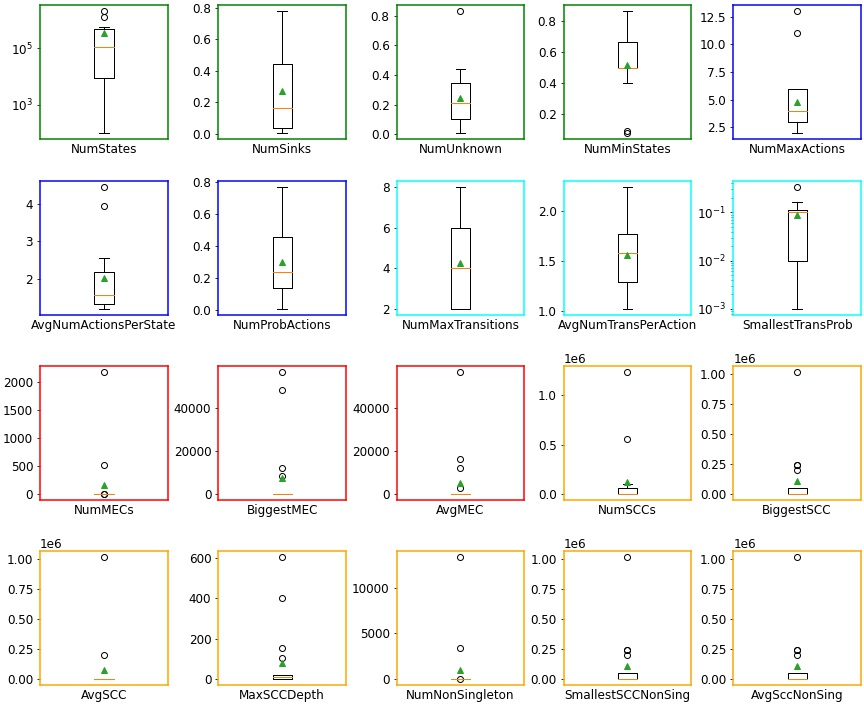
\includegraphics[width=1\textwidth]{figures/Real_FeatureDistribution.jpg}
    \caption[Feature Distribution of the case studies]{
        A Box plot of the feature distribution of the real case studies. The description on how to read the plot is provided in Section \ref{plot:boxplot}.
    }
    \label{fig:Real_FeatureDistribution}
\end{figure}
The box plot provides the following insights:
\begin{itemize} \label{insights:realDistribution}
    \item According to AvgNumActionsPerState and AvgNumTransPerAction, models have on average 2 actions per state and 1.5 transitions per action
    \item According to NumUnknown, on average 80\% of the states of the models are trivial, and their value is computed with simple graph algorithms 
    \item Generally, the number of states is evenly split between Maximizer and Minimizer
    \item According to NumProbActions, usually around 70 to 85\% of all actions are deterministic
    \item According to NumMECs, most models do not contain end components
\end{itemize}

By furthermore printing the maximal and minimal occurring values of each feature we obtain that the smallest occurring transition probability is 0.001.

We also use the information to draw conclusions about which structural cases do not appear in the real case studies. 
None of the models contain these cases: \textcolor{purple}{Leave out? No real gain here}
\begin{itemize}
    \item Models with numerous actions per state
    \item Models with numerous Transitions per action
    \item Models with very small transition probabilities
\end{itemize}
\FloatBarrier
Furthermore, we use box plots to evaluate for which features our random generation algorithm from Chapter \ref{ch:randomGen} is biased.
Figure \ref{fig:Random_FeatureDistribution} contains the box plots for our randomly generated models.
\begin{figure}[h!]
    \centering
    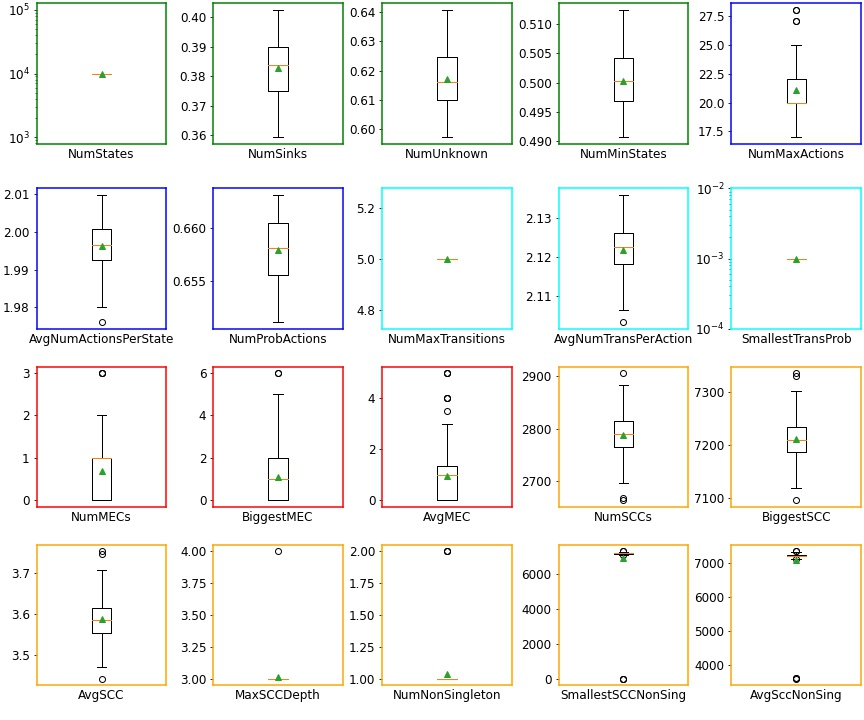
\includegraphics[width=1\textwidth]{figures/RandomRandom_FeatureDistribution.jpg}
    \caption[Feature Distribution of random models]{
        A Box plot of the feature Distribution of models generated randomly with Algorithm \ref{alg:randomRandom}. The description on how to read the plot is provided in Section \ref{plot:boxplot}.
        %The evaluation of the plot is located in Section \ref{insights:randomRandom}.
    }
    \label{fig:Random_FeatureDistribution}
\end{figure}
\FloatBarrier

The biases we read from this plot are:
\begin{itemize} \label{insights:randomRandom}
    \item On average, 38.5\% of the values of states of the models are computed by trivial graph algorithms. NumSinks shows that almost all known states are sinks.
    \item With the chosen parameters, our algorithm generates models with 2 actions per state on average
     and 2 transitions per action on average.     
     However, our parameters allows us to change the number of actions and transitions per state.
    \item NumNonSingleton shows that in almost all cases there is only one strongly connected component.
        This is because we uniformly randomize where a transition may lead. Thus, it is likely that big SCCs are formed. 
        If necessary, the RandomSCC guideline can control the size of the SCCs.
    \item NumMECs indicates that there is usually either one MEC or none at all. Also, the MECs tend to have very few states (usually no more than 2).
    However, there are parameter configurations such that we form bigger MECs. For example setting the parameters in such a way that the actions are deterministic
    and adding an action to every state in the backwards procedure of Algorithm \ref{alg:randomRandom} creates models with a high tendency of forming few MECs that usually contain the whole state-space.
    Nevertheless, without providing a specific guideline, we have very limited control over the number and size of the MECs.
    \item Our random generation algorithm introduces a bias towards various properties like the number of SCCs or the average number of transitions per action.
    While on average models have only two actions, the maximal number of actions a state has is usually between 20 and 22.
    When analyzing the number of actions in relation to the state index, states with many actions always have low indices.
\end{itemize}

When comparing the feature distributions of the real case studies and the distributions of the models generated by Algorithm \ref{alg:randomRandom},
they have similar biases for many features. Both benchmarks tend to have few big SCCs, few actions per state, and few transitions per action.
However, we are not restricted to creating models similar to the current case studies. The number of actions and transitions can be adjusted by parameters,
and the way in which SCCs are formed can be influenced by guidelines as described in Section \ref{sec:guidelines}.

To demonstrate this, we present in Figure \ref{fig:RandomSCC_FeatureDistributions} the feature distribution of a set of models we have created by using the RandomSCC guideline.
We use the same parameters to create the models as for the set displayed in Figure \ref{fig:Random_FeatureDistribution}, but change 
the number of actions to \textcolor{red}{Parameter}.
Figure \ref{fig:Random_FeatureDistribution} contains the box plots for our randomly generated models.
\begin{figure}[h!]
    \centering
    
\includegraphics[width=1\textwidth]{figures/Placeholder.png}
    \caption[Feature Distribution of random models]{
        Feature Distribution of randomly generated models by applying the RandomSCC guideline. For a description on how to read the plot is provided in Section \ref{plot:boxplot}.
        The evaluation of the plot is located in Section \ref{insights:sccDistribution}.
    }
    \label{fig:RandomSCC_FeatureDistributions}
\end{figure}
\FloatBarrier

\label{insights:sccDistribution}
\textcolor{red}{Some easy conclusions. Cleary different - smaller SCCs, more actions, hopefully less bias towards states with smaller index}

\subsubsection*{Increasing the number of unknown states}
A reoccurring problem we encountered was that many models we generated randomly were solved entirely or mostly by simple graph algorithms.
While in models generated by Algorithm \ref{alg:randomRandom} over 60\% of the states could not be computed during precomputation, 
for the guidelines RandomSCC and RandomTree on average less than 10\% of the state space could not be computed trivially.
If the entire or most of the state space is precomputed, the resulting problem is usually too easy to draw meaningful conclusions from it.
To artificially make the problems generated through RandomSCC and RandomTree harder, we set the forceUnknown switch to true. 
At the moment this is equivalently to disabling the computation of 
states that can surely reach the target. \textcolor{purple}{So then the question is why didnt we just do that?
Because setting the value to 0.9 is a realistic scenario. There can be models that have value 1 only in the target. 
But this feels like a stupid way of justifying this switch. In the end the states are still kinda trivial, right?}
The low Unknown\% is mostly due to large parts of the state space being unable to ever reach a target.


\section{Algorithm comparison results}

In this section, we compare the Algorithms introduced in Section \ref{sec:SGAlgos} on real case studies, handcrafted examples, and our randomly generated models to both evaluate the 
performance of the algorithms relative to each other and find correlations between model feature values and algorithm performance.

First, we provide a general overview of the performance of all algorithms on our benchmarking set through a line plot in Figure \ref{fig:AlgoPerformance}.
\begin{figure}[h!]
    \centering
    \subfloat[\centering Accumulated algorithm performance overview on real case studies]{{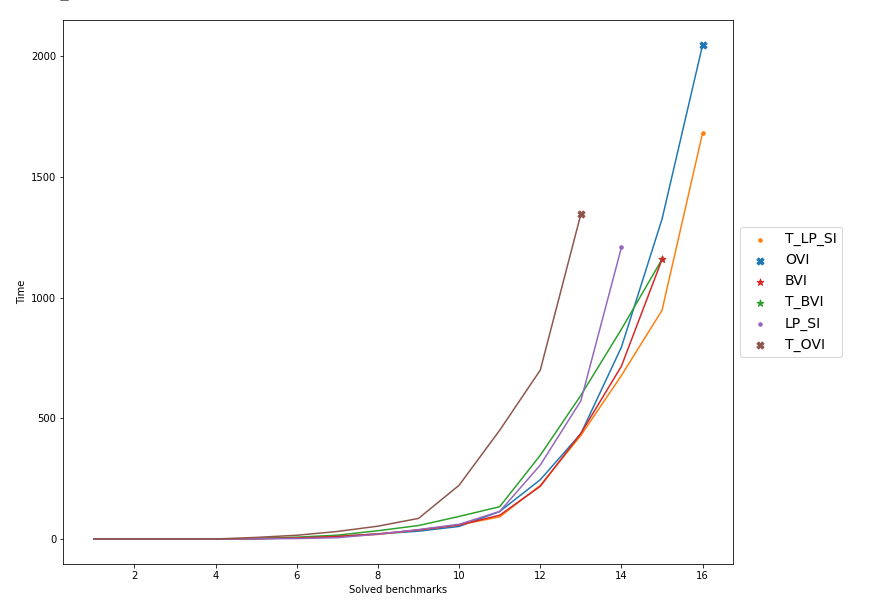
\includegraphics[width=0.7\textwidth]{figures/Real_AlgoPerformance.png} }}%
    \qquad
    \subfloat[\centering Accumulated algorithm performance overview on all randomly generated models.]{{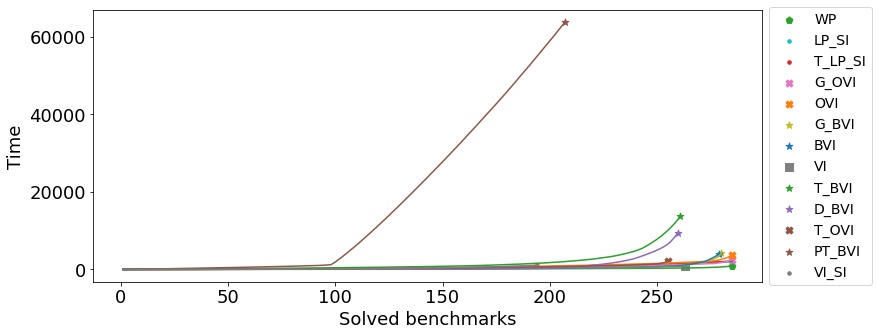
\includegraphics[width=0.7\textwidth]{figures/RandomRandom_AlgoPerformance.png} }}%
    \caption[Overview of Algorithm Performance]{
        A line plot providing an overview of the accumulated algorithm performance.
        }%
    \label{fig:AlgoPerformance}
\end{figure}

%For value-iteration-based algorithms, we provide the same graph with the number of iterations required to solve the models on the y-axis in Figure
%\ref{fig:AlgoPerformanceIters} \textcolor{red}{Add star-graph for iterations}.

\textcolor{red}{split into real case studies (Figure 7.3a) and randomly generated models (Figure 7.3b)}We read several clues from Figure \ref{fig:AlgoPerformance}:
$\WP$, $\OVI$, and $\TLPSI$ seem to be the most performant algorithms for our benchmarks.

We split our analysis into three subtopics: 
First, we compare the three value-iteration-based algorithms with guarantees $\OVI$, $\WP$, and $\BVI$. 
Then, we analyze the impact of the optimizations from Subsection \ref{subsec:optimizations} on their respective baseline algorithms.
Lastly, we investigate the performance of strategy-iteration-based algorithms in comparison to value-iteration-based algorithms.
For $\OVI$, $\WP$, $\BVI$ and their optimizations, we compare the number of iterations required to solve a model in addition to the time.
While time is practically more relevant, the number of iterations is independent of how optimized the implementation of the algorithm is.
\FloatBarrier

\subsection{$\BVI$ vs $\OVI$ vs $\WP$}
We read from Figure \ref{fig:AlgoPerformance} that WP is the fastest to solve the problems on both randomly generated models and real case studies.
To see whether this is the case for all models or only when accumulating runtime, we provide a scatter plot in Figure \ref{fig:WPvsBVIvsOVI}.
The x-axis marks the time $\WP$ requires to solve a stochastic game, and the y-axis marks the respective time $\BVI$ or $\OVI$ needs.
The two lines next to the diagonal mark the case that $\WP$ is twice as fast as $\BVI$ / $\OVI$ or half as fast.

\begin{figure}[h!]
    \centering
    \subfloat[\centering Time required to solve a model]{{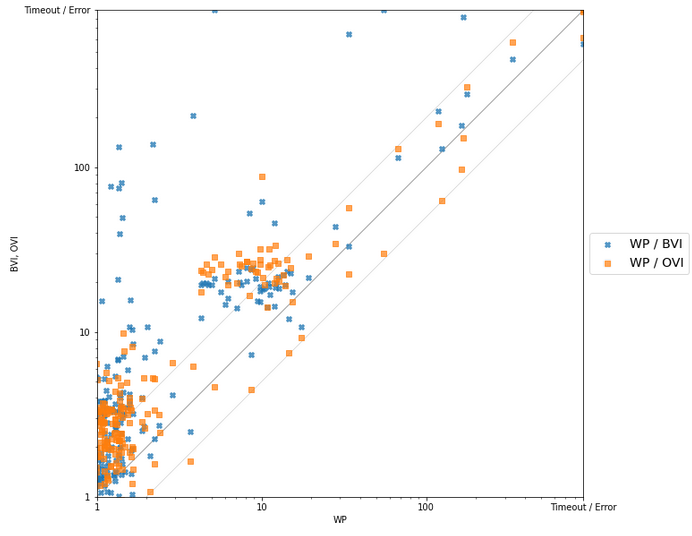
\includegraphics[width=.48\textwidth]{figures/WPvsBVIandOVIonAll.png} }}%
    \
    \subfloat[\centering Iterations required to solve a model]{{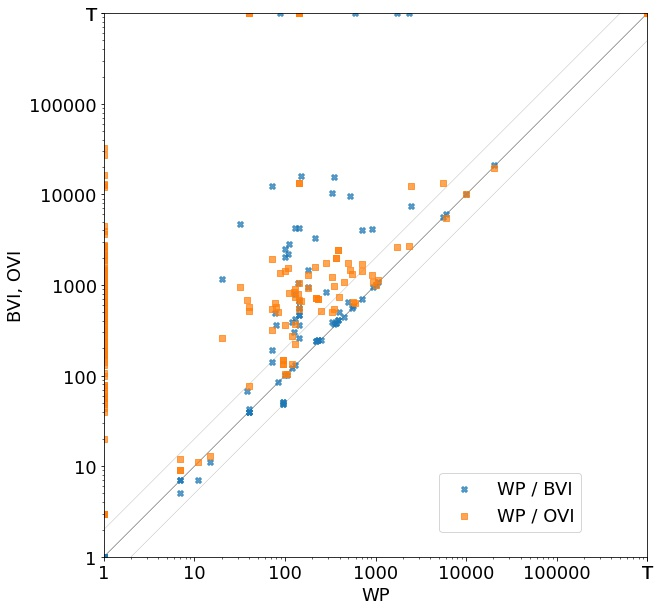
\includegraphics[width=.48\textwidth]{figures/WPvsBVIandOVIonAll_Iters.png} }}%
    \caption{$\WP$ compared to $\BVI$ and $\OVI$ on every model of all datasets. See \ref{plot:performanceScatter} for a reference on how to read the plot.}%
    \label{fig:WPvsBVIvsOVI}%
    \end{figure}
\FloatBarrier

\subsubsection*{$\WP$}
Regarding time, $\WP$ is neither significantly better nor worse than $\OVI$ and $\BVI$.
However, in every data set we analyzed, $\WP$ was one of the fast algorithms when measuring accumulated time.
On large models, $\WP$ was accumulated slower than $\BVI$, but they are close enough that the difference is negligible.
When comparing iterations, $\WP$ requires almost always fewer iterations than $\BVI$ and $\OVI$, and never more than twice as many.

Since we could not find a clear weakness of $\WP$, we conclude that it is a good initial choice in case of doubt.

\iffalse
Regarding time, $\WP$ is usually faster than $\BVI$ and $\OVI$ and never requires more than twice as long.
We are interested in whether there is a correlation between structural properties and $\WP$ being better or worse than the other two.
To inspect the cases where $\WP$ is better than $\OVI$ or the other way around, we plot the feature of the models where one algorithm was at least
1.5 times faster than the other one. Figure \ref{fig:WPvsOVIon1DFeatureScatter} visualizes these cases. 
The red dots mark models where $\OVI$ is at least 1.5 times faster than $\WP$, and the green dots mark models where $\WP$ is at least 1.5 times faster than $\OVI$.
The x-axis displays the range of values that occur for the feature. 
If the dots are clustered for a feature, either one algorithm was only faster if the model had this kind of structural composition, 
or there are only discrete values available for the feature. For example, the number of states is mostly discrete because the random models depend on an input parameter.

\begin{figure}[t]
    \centering
    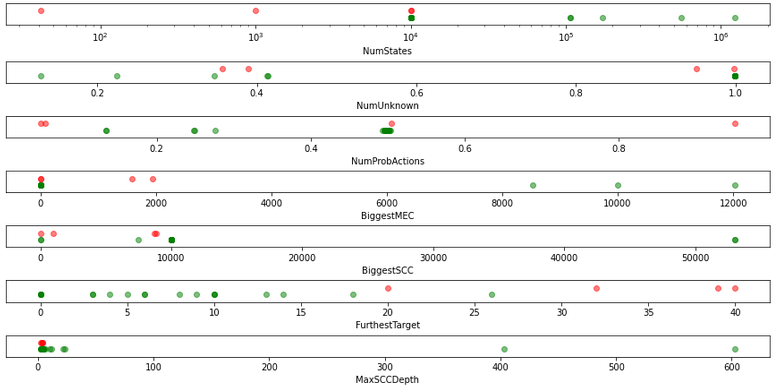
\includegraphics[width=1\textwidth]{figures/WPvsOVIon1DFeatureScatter.png}
    \caption[$\WP$ compared to $\OVI$]{
        The red dots mark models where $\OVI$ is at least 1.5 times faster than $\WP$, and the green dots mark models where $\WP$ is at least 1.5 times faster than $\OVI$.
        The x-axis displays the range of values that occur for the feature. 
        If the dots are clustered for a feature, either one algorithm was only faster if the model had this kind of structural composition, 
        or there are only discrete values available for the feature. For example, the number of states is mostly discrete because the random models depend on an input parameter.
    }
    \label{fig:WPvsOVIon1DFeatureScatter}
\end{figure}

According to Figure \ref{fig:WPvsOVIon1DFeatureScatter}, $\WP$ was better than $\OVI$ if the model had more states, had big MECs and big SCCs.
$\OVI$ seems to be better if the furthest target is far away from the initial state, but since we cannot tie this to any structural significant property,
it may also be noise. If this interpretation is correct, $\WP$ should become even better than $\OVI$ if we use larger models.

The same plot for $\WP$ and $\BVI$ is harder to interpret since there are only two cases where $\BVI$ is 1.5 times faster than $\OVI$, and 40 cases
for the opposite event. Thus, we conclude that $\WP$ is overall more performant on our benchmarks than $\BVI$ regarding runtime. 
\textcolor{blue}{@Maxi: The two cases where BVI is better are quite noisy, so it is not worth including the Figure in my Opinion.
But I have added it in case you think it is interesting. It is Figure \ref{fig:WPvsBVIon1DFeatureScatter}}
\fi

\subsubsection*{$\BVI$}

Figure \ref{fig:BVIvsWPvsOVI} provides an overview of the time $\BVI$ requires to solve a model compared to $\OVI$ and $\WP$.
While both the accumulated runtime of Figure \ref{fig:AlgoPerformance} and the left scatter plot with all the models of Figure \ref{fig:BVIvsWPvsOVI}
suggest that for more complicated models $\OVI$ and $\WP$ are faster than $\BVI$, the times required to solve large models only in Figure \ref{fig:BVIvsWPvsOVI} (b)
shows that for large models $\BVI$ tends to be faster. \textcolor{purple}{However, we emphasize that this tendency may be due to a lack of large models.}

\begin{figure}[h!]
    \centering
    \subfloat[\centering Time required to solve on every model of all datasets]{{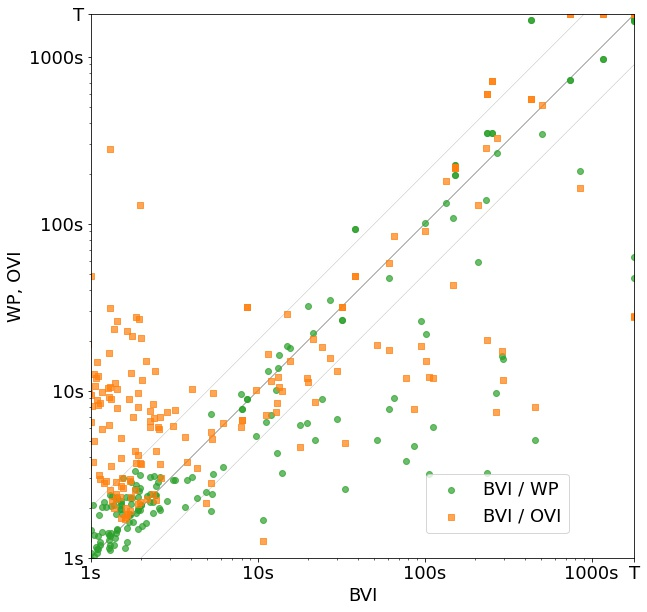
\includegraphics[width=.48\textwidth]{figures/BVIvsWPvsOVI.jpg} }}%
    \
    \subfloat[\centering Time required to solve a model only with large models ]{{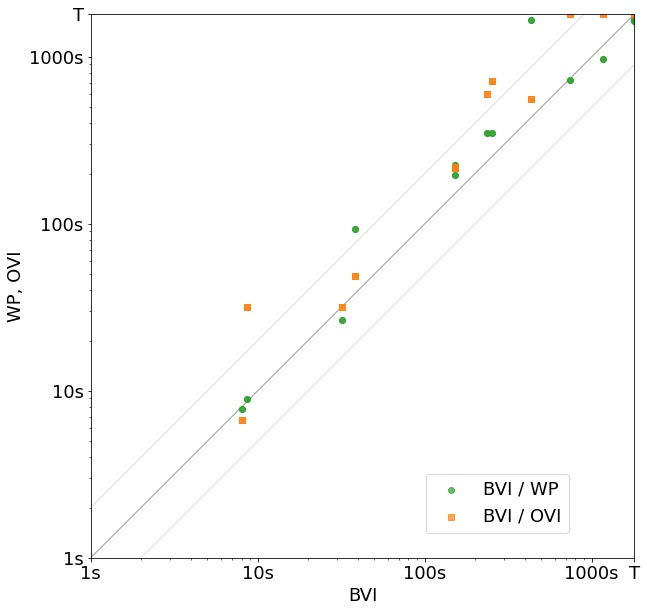
\includegraphics[width=.48\textwidth]{figures/BVIvsWPvsOVI_OnlyBig.jpg} }}%
    \caption{$\BVI$ compared to $\WP$ and $\OVI$. See \ref{plot:performanceScatter} for a reference on how to read the plot.}%
    \label{fig:BVIvsWPvsOVI}%
    \end{figure}
\FloatBarrier

We found that $\BVI$ usually requires fewer iterations than $\OVI$ to solve a model. 
\textcolor{red}{I do have an image of that, but it is probably not interesting to see. Appendix or leave out?}

\subsubsection*{$\OVI$}
While $\OVI$ seems very performant when looking at accumulated runtime, Figure \ref{fig:BVIvsWPvsOVI} and \textcolor{purple}{Ref Large models} provide evidence that it requires more time than $\BVI$ and $\OVI$ for large models.
This is due to the termination criterion of $\OVI$: 
If no value improves more than an $\epsilon'$, the verification phase starts to ensure that $\OVI$ is close enough to the optimal value.
If the verification fails, $\epsilon'$ is halved. 
Thus, it is possible that the verification phase fails, although the game is almost solved.
In that case $\OVI$ will iterate unnecessary extra steps until it reaches its new precision that verifies that $\OVI$ may indeed terminate.
For large models, it is likelier that a model is so complex that it requires multiple verification phases as Figure
\textcolor{red}{Show something about verification phases (or do not)} suggests. 
Thus, it is also more probable that the precision is halved at a point that will lead to unnecessary iterations.
In addition to that iterations are also more costly for larger models since the state space is bigger.

$\OVI$ generally requires more iterations than $\WP$ and $\BVI$. This is partly because of the extra iterations that may happen in $\OVI$ as mentioned, 
and partly because during verification phase only the upper bound is being iterated on. Meanwhile, in $\BVI$ both upper- and lower bound are updated per iteration.
Also, it is interesting to see that for about half of the models in Figure \ref{fig:WPvsBVIvsOVI} $\WP$ requires only 1 iteration whereas $\OVI$ requires many iterations to solve the model.
The red dots in Figure \ref{fig:OVIinstantCompute} visualize the value of the games where $\WP$ required only 1 iteration and $\OVI$ multiple,
while the green dots represent models where $\WP$ required also multiple iterations to solve the game.

\begin{figure}[h!]
    \centering
    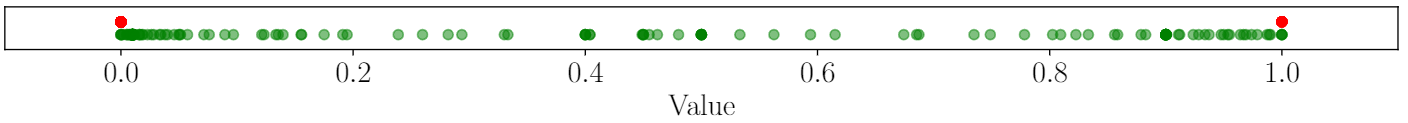
\includegraphics[width=1\textwidth]{figures/OVI_Bad_At_Computing_Instant_Values.png}
    \caption[$\OVI$ cannot instantly compute models]{
        A one dimensional scatter plot of when $\WP$ could solve a model in 1 iteration while $\OVI$ could not (red) 
        against where $\WP$ requires more than 1 iteration (green).
    }
    \label{fig:OVIinstantCompute}
\end{figure}
\FloatBarrier

Clearly, in some instances where a game has value 0 or 1, $\WP$ is able to identify its value in only 1 iteration while $\OVI$ cannot.
$\BVI$ is also capable of solving these models in 1 iteration. \textcolor{purple}{Ref to BVI scatter}
In the runtime scatter plot of Figure \ref{fig:WPvsBVIvsOVI}, these models are the cloud of orange dots in the lower left quadrant \textcolor{red}{Is that true?}.
However, even if $\BVI$ and $\WP$ require only one iteration, they still require up to 5 seconds to perform this iteration.

\textcolor{red}{I could talk about best-case OVI examples one action leading to target with 0.5 in every state and the other into the chain with self loop.}

\subsection{Analyzing the optimizations}

Figure \ref{fig:AlgoPerformance} indicated that optimizations introduced in Subsection \ref{subsec:optimizations} do not always improve the accumulated runtime. 
For example, while $\BVID$ is better than $\BVI$ in the real case studies, it is significantly worse on our randomly generated models.
To analyze the effect of the optimizations, we compare $\BVI$, $\OVI$, and $\LPSI$ with the optimizations that apply to them in scatter plots.
To each optimization, we provide a scatter plot with time required to solve the models, and one scatter plot with iterations required to solve the models.
For the iterations scatter plots we include only $\BVI$ and $\OVI$ since iterations in strategy iteration are not comparable to iterations in value iteration.

$\mathbf{Gauss-Seidel}$ for $\BVI$:
\begin{figure}[h!]
    \centering
    \subfloat[\centering Time required to solve a model]{{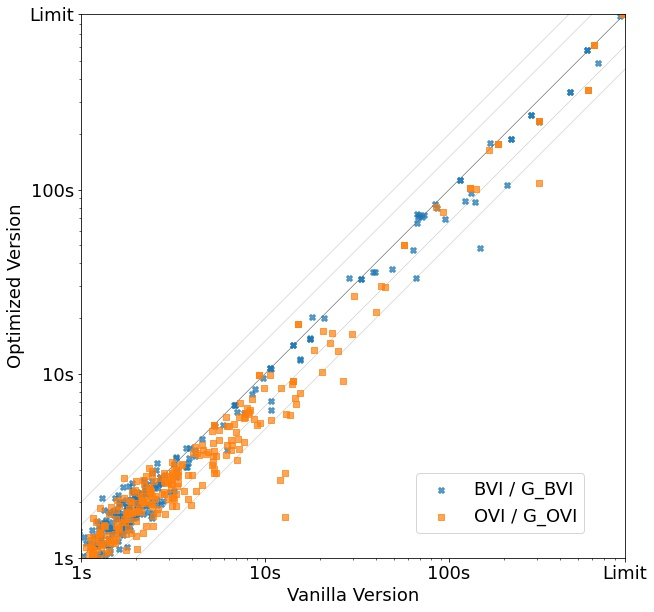
\includegraphics[width=.48\textwidth]{figures/Scatter_G.jpg} }}%
    \
    \subfloat[\centering Iterations required to solve a model]{{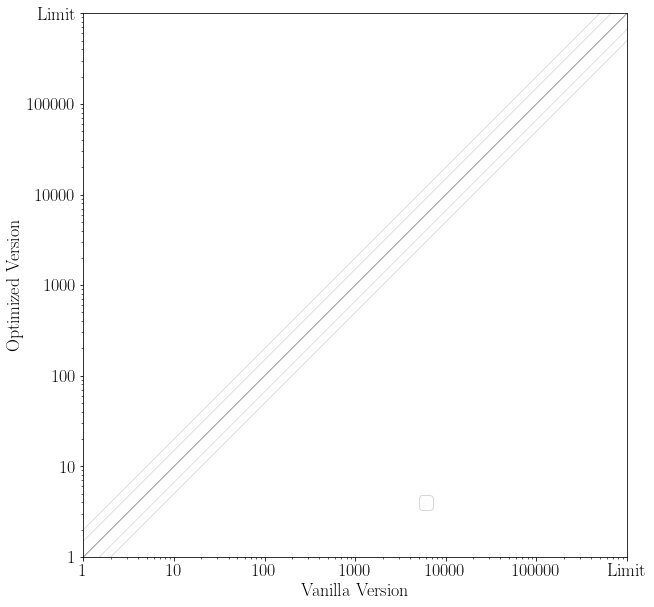
\includegraphics[width=.48\textwidth]{figures/Scatter_G_iters.jpg} }}%
    \caption{$\BVI$ and $\OVI$ compared to their Gauss-Seidel optimizations on every model of all datasets}%
    \label{fig:Scatter_G}%
    \end{figure}
\FloatBarrier

\textcolor{red}{CAREFUL! For big models this may be untrue}
As Figure \ref{fig:Scatter_G} suggests, using the Gauss-Seidel optimization may reduce both the time and iterations required to solve a model by 1-4 times in most cases.
However, Figure \ref{fig:AlgoPerformance} shows when accumulating runtime, $\OVI$ is still slightly faster than $\OVIG$.
The Gauss-Seidel optimization is slower in some cases because the values are computed state by state to enable using already computed results.
The unoptimized version uses vector operations instead, which turn out to be faster sometimes.
Furthermore, it is possible that there are more iterations required to solve. 
This is because $\OVI$ and $\BVI$ may find different end components to deflate depending on whether Gauss-Seidel is used or not.
In some cases, the unoptimized version is able to find more favorable sets of end components and requires thus less iterations.
Changing the order of computation of the states for the Gauss-Seidel optimization by computing along a topological enumeration of the states did not
yield improvements in our experiments.  

\textcolor{purple}{Probably, Gauss-Seidel should be even worse for bigger models since there is more room for "not paying off" using state-by-state computation.}


$\mathbf{D}$ for $\BVI$:
\begin{figure}[h!]
    \centering
    \subfloat[\centering Time required to solve a model]{{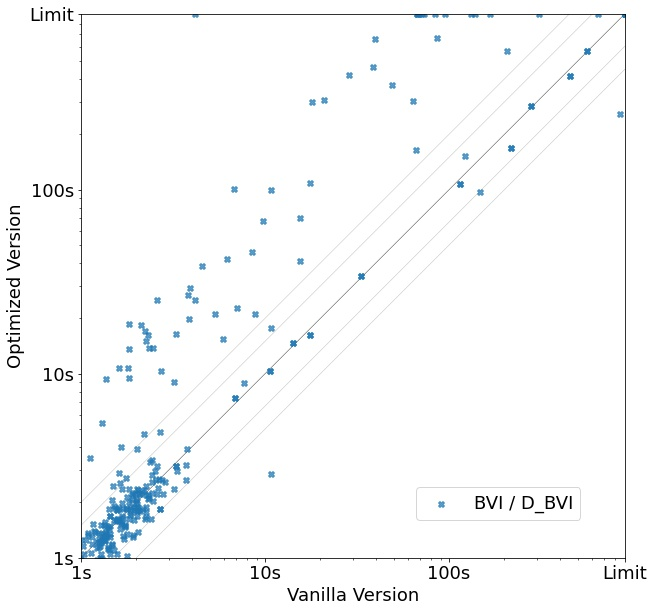
\includegraphics[width=.48\textwidth]{figures/Scatter_D.jpg} }}%
    \
    \subfloat[\centering Iterations required to solve a model]{{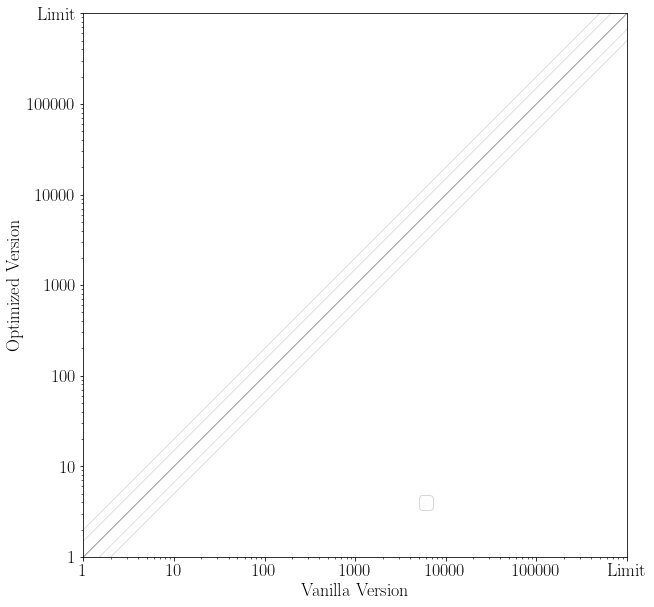
\includegraphics[width=.48\textwidth]{figures/Scatter_D_iters.jpg} }}%
    \caption{$\BVI$ compared to its optimization where deflating happens only every 100 iterations on every model of all datasets}%
    \label{fig:Scatter_D}%
    \end{figure}
\FloatBarrier
Figure \ref{fig:Scatter_D} clearly indicates that although $\BVID$ may solve sometimes models faster, 
for most of our models it could not compete with $\BVI$.

$\mathbf{T}$ for $\BVI, \OVI$ and $\LPSI$:
\begin{figure}[h!]
    \centering
    \subfloat[\centering Time required to solve a model]{{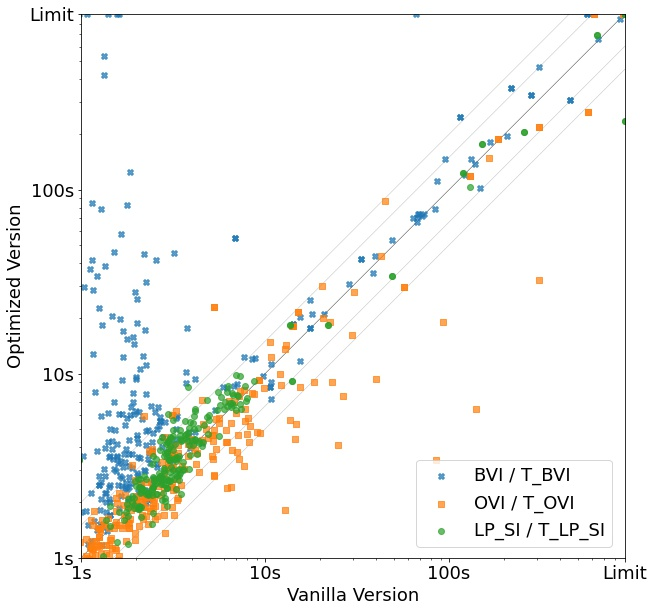
\includegraphics[width=.48\textwidth]{figures/Scatter_T.jpg} }}%
    \
    \subfloat[\centering Iterations required to solve a model]{{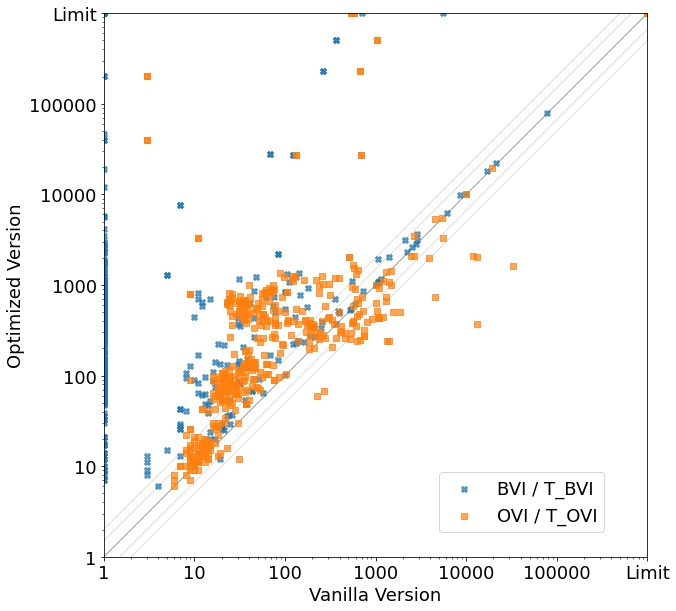
\includegraphics[width=.48\textwidth]{figures/Scatter_T_iters.jpg} }}%
    \caption{$\BVI$, $\OVI$ and $\LPSI$ compared to their topological optimizations on every model of all datasets}%
    \label{fig:Scatter_T}%
    \end{figure}
\FloatBarrier

As the scatter plot \ref{fig:Scatter_T} shows,
the topological addition for strategy iteration with linear programming in the real case studies and random models does 
neither in- nor decrease the performance of the algorithm considerably.
However, most models have very few SCCs, so the topological optimization does not contribute a lot.
The data point where $\TLPSI$ is significantly faster is on the real case study "dice", where every state is an SCC on its own.
This is obviously the best-case scenario for topological algorithms.
\textcolor{red}{Show Scatter.
Explain why $\OVI$ and $\BVI$ do not scale that well (explained in Gandalf Paper)}

\textcolor{red}{When comparing $\OVI$ with $\OVI_T$ I could not find any defining feature that would say much}

$\TOPAlg$ for $\BVI$:

$\TOPAlg$ seems to perform worse than $\BVI$ in general. This is because we solve the DTMCs with exact methods. 
\textcolor{red}{Scatter BVI vs TOP.}
This requires a matrix inversion, which is an $\mathcal{O}(n^{2})$-operation, where n is the number of states in the SCC whose value is being computed.
The bottleneck becomes apparent if we consider a scatter plot where we show the runtime against the size of the biggest SCC as in Figure \ref{fig:} \textcolor{red}{ADD FEATURE-SCATTER}.
We have also tried solving the resulting MDP with linear programming instead of strategy iteration, but it was still worse than $\TLPSI$.

%There are several relations we read from Figure \ref{fig:AlgoPerformance}:
%\begin{itemize}
%    \item $\TLPSI$ is accumulated better than $\LPSI$.
%    \item $\TLPSI$ is performant for small models
%    \item $\WP$ is usually the best value iteration approach
%    \item $\OVI$ is usually better than $\BVI$ for small models
%    \item $\TOPAlg$ does not seem very promising
%    \item The optimizations do not seem to do much except for the topological switch for $\TLPSI$ and $\WP$
%    \item Why GBVI is not always better than BVI (iterationwise)
%\end{itemize}

\subsection{Algorithms based on strategy iteration}
\textcolor{red}{It would also be interesting to see if more probabilistic loops affect $\LPSI$ as strong as VI}.

Although value iteration was regarded for a long time to be the most performant algorithm type for solving stochastic games, 
\cite{gandalf} that $\SI$ is a valid option, and that mathematical programming can be good sometimes.
Thus, in addition to $\SI$ we consider $\SISI$ and $\LPSI$ which do not use value iteration at all to solve stochastic games.

\subsubsection*{Strategy iteration with linear programming}
$\TLPSI$ yielded the best results alongside widest-path bounded value iteration.
Since strategy iteration simply tries to make an informed decision on which strategy to pick and solves the underlying MDP, 
we have to inspect the algorithms we use to solve MDPs - for $\TLPSI$ this is linear programming.

Linear programming scales worse than value iteration for huge models.
As Figure \textcolor{red}{REF BIG MODELS} indicates, $\TLPSI$ and $\LPSI$ were slower to solve the models than $\OVI$, $\BVI$ and $\WP$.
This is partly due to the LP solver running out of memory, which happened 8/36. \textcolor{red}{Check that this number is correct.}

\textcolor{purple}{To test this, we have 
run several benchmarks on models with state size 10 million and varying SCC sizes. [Now enter Feature-Performance Scatter Plot] 
The bigger the SCCs become, the slower $\TLPSI$ becomes. At a size of [...] per SCC, $\WP$ was faster than $\TLPSI$.}
Thus, we do not recommend using $\TLPSI$ on models with numerous states.
However, $\TLPSI$ may be a good complementary solution approach in case a model is especially hard for value iteration.
Also, the topological improvement allows solving models with huge numbers of small SCCs faster than value iteration.
\textcolor{purple}{And also value iteration was the focus of research for the last 20 years. 
LP could likely be improved. At the moment, we do not even deflate but use MIP to encode the maximum-best-exit constraints. But this should maybe go into future work}

\subsubsection*{Strategy iteration with exact Markov chain solving}
\textcolor{purple}{Just bad. Fails most of the time because either out of memory or timeout. 
While $\TOPAlg$ needs to perform exact DTMC solving only once per SCC and $\TOPAlg$ is already not so great, $\SISI$ may change strategies and thus needs to perform exact DTMC solving multiple times.
}

\subsubsection*{Strategy iteration with value iteration}
\textcolor{purple}{In general okay but worse than $\BVI$. Will usually struggle where value iteration struggles in general.}


\subsection{Big models}
\textcolor{red}{Might also put in somewhere else. Basically too little data but also pretty though PRISM constraints.
$\TLPSI$ ran sometimes out of stack (see memo comparation in GANDALF for QP or make own) suggesting that $\LPSI$ may not scale too well 
for bigger models but it may be good if there are many SCCs with smaller SCCs.
It seems that $\OVI$ does not scale too well. However, in the end it is very important to note that we are lacking the capacity to create
big models.}


\iffalse
\section{Searching correlations between algorithms and features}
Lastly, we are interested in correlations between algorithm performance and values of features.
Ideally, we would like to find cases where one algorithm scales better with certain features than others.
If we were to find enough such correlations, it would be possible to implement an efficient portfolio solver, which
would analyze the graph structure and decide based on the feature values which algorithm is most likely the best one to use in this case.
To find these correlations, we use the following visualization tools:

\textcolor{purple}{I am not really sure what I want to do with this section. 
But it would be a cool place to show algorithm-feature correlations and to show the ideas we applied to search for correlations.
Maybe I should instead make a separate section with all graph types that is easy to look up.}

\textcolor{red}{Maybe search for some scatters where the algorithms differ a lot and show them.}

\subparagraph*{Heatmaps}
Heatmaps visualize correlation matrices - matrices where one feature is mapped against another. The higher the correlation value, the stronger
a correlation between two features is. On the diagonal of the matrix, the correlation is maximal since there is a directly proportional correlation between
a feature and itself. Ideally, we would like to get clues from the heatmap which features or correlations we should investigate.
However, for the most part, we could not gather any non-trivial information from heatmaps. \textcolor{purple}{This is also tricky because
there is only one type of correlation that can be shown effectively: Most often we search for linear correlation with heatmaps. Thus,
if one feature depends in a non-linear fashion on another - for example if it rises quadratically - the correlation value may still be very low.}

\subparagraph*{Feature-performace scatter plots}
We plot algorithm runtime / iterations against feature values.

What is there to find in these graphs?
\begin{itemize}
    \item Clearly visible how TOP scales with SCC-size
    \item All scale with number of unknowns, which is no surprise but might be mentioned.
\end{itemize}

\subparagraph*{One dimensional scatter plots for features}
We can define two events A, B. Then we get models where A happens, models where B happens and then plot the feature values for models that are in set A or set B.
This way, we can find clusters and make conclusions like "If A happens, then the models have these feature values."
\fi